\documentclass[12pt]{exam}

\usepackage{ge05}
\usepackage{comment}
\usepackage{graphicx}
\usepackage[dvipdfm]{hyperref}
\urlstyle{rm}   % change fonts for url's (from Chad Jones)
\hypersetup{
    colorlinks=true,        % kills boxes
    allcolors=blue,
    pdfsubject={NYU Stern course GB 2303, Global Economy},
    pdfauthor={Dave Backus @ NYU},
    pdfstartview={FitH},
    pdfpagemode={UseNone},
%    pdfnewwindow=true,      % links in new window
%    linkcolor=blue,         % color of internal links
%    citecolor=blue,         % color of links to bibliography
%    filecolor=blue,         % color of file links
%    urlcolor=blue           % color of external links
% see:  http://www.tug.org/applications/hyperref/manual.html
}

% for ge05.sty
\def\ClassName{The Global Economy}
%\def\Category{Professor David Backus}
\def\Category{Backus \& Cooley}
\def\HeadName{Problem Set \#1}
\newcommand{\phm}{\phantom{--}}
\newcommand{\NX}{\mbox{\it NX\/}}

\printanswers

\begin{document}
\parindent = 0.0in
\parskip = \bigskipamount
\thispagestyle{empty}%
\Head

\centerline{\large \bf \HeadName: Macroeconomic Data}
\centerline{Revised:  \today}

\medskip
{\it You may do this assignment in a group of up to five people.
Whatever you hand in should be the work of your group.}

\begin{questions}

\begin{solution}
Brief answers follow,
but see also the spreadsheet posted on the course website.
\end{solution}

% --------------------------------------------------------------------
\question National accounts in Margaritaville (40 points).
Jimmy Buffett has decided to apply for membership in the European Union
on behalf of his newly sovereign nation, Margaritaville.
As part of his application, he must provide the EU
technocrats with a complete set of national accounts.
You have been hired as the Chief National Accountant.
Your first day on the job,
you receive an official Coral Reefer Crew{\texttrademark} t-shirt
and the following information about local economic activity:
%
\begin{itemize}
\item Local Cheeseburger in Paradise{\texttrademark} cafes
sold \$50,000 worth of cheeseburgers to local consumers.
Their expenses were:  imported beef and sesame seeds (\$7,000),
locally produced catsup (\$10,000),
wages and benefits (\$20,000), and rent (\$3,000).
Hint: you will need to compute the profit earned by the cafes.

\item Local tomato growers sold \$8,000 worth of tomatoes to domestic
catsup producers and exported another \$2,000 to the US.
They paid land rent (\$1,000) and wages (\$9,000).

\item Local producers of the Margaritaville Frozen Concoction Maker{\texttrademark }
sold \$100,000 worth of blenders.
40\% were exported to Europe, the remainder to local consumers.
Their expenses were \$15,000 worth of imported metal,
\$15,000 for a new CNC machine imported from Germany,
and \$70,000 in wages.

\item The domestic catsup industry sold \$10,000 worth of product to local
cafes.
They purchased \$8,000 worth of tomatoes from domestic growers
and paid \$2,000 in wages.


\item The newly-formed government collected \$10,000 in taxes from its citizens
and paid \$10,000 to government regulators, who oversee food and beverage safety.
\end{itemize}
%
You mission is to use this raw data to construct
national income and product accounts for Magaritaville.
Specifically:
%
\begin{parts}
\part Compute GDP and its expenditure components (consumption,
investment, government purchases of goods and services,
exports, and imports).
(10~points)

\part What are saving and investment?  Why are they different?
Where does the difference go?
(10~points)

\part Compute the contribution of each production unit to GDP.
(10~points)

\part Jimmy looks over your calculation in (a) and is worried
that you made a mistake.
Over a couple Land Shark Lagers{\texttrademark}
you explain to him that GDP can be computed three different ways:
the sum of value-added across production units (Gross Domestic Product),
the sum of expenditure components (Gross Domestic Expenditure),
and the sum of payments to labor and capital (Gross Domestic Income).
You do the remaining one, payments to labor and capital,
and show him that you get the same answer.
He buys you a margarita to show his appreciation.
(10~points)
\end{parts}

\begin{solution}
It's easiest to do the whole thing on a spreadsheet --- see the link on
the course website.
The idea is to calculate value added, income, and final sales,
as we did in class.
The two new wrinkles are government production,
which is valued at cost (income = value added),
and investment,
which is not counted as an expense.
There's more on both in the notes.

Here's a quick overview organized by producer:
\begin{itemize}
\item Cafes:  Value added comes from
sales of 50 minus intermediate goods of 17,
which gives you value-added of 33.
On the income side this corresponds to 20 to labor, 3 in rent, and 10 of profit
to the owner.
All of the sales revenue is final sales to consumers.
How do we handle the input of imported beef and seeds?
One approach is to put a 7 in imports.
The approach we follow in the spreadsheet is to introduce
and extra production unit which sells beef and seeds to us.
They give us the same answer.
\item Tomatoes:  Value added is 10, which equals
income of 10 (9 to labor, 1 to rent).
Only the exports of 2 counts as final sales,
the rest is an input to the catsup producer.
\item MFCM:  Value added is sales of 100 minus the 15 of metal,
for a total of 85.
By convention, we do not include the 15 of new machines as an expense,
because it's an investment in new plant and equipment.
On the income side, that consists of wages of 70 and profit of 15.
Finals sales includes consumption of 60, exports of 40, imports of 30,
and investment of 15.
The investment really goes with the machine producer,
which is how it's listed in the spreadsheet:  an investment of 15
and an import (for us, export for the machine producer) of 15.
\item Catsup:  Revenue of 10 minus intermediate inputs of 8
gives us value-added of 2, which is paid as wages.
None of it counts as final sales, since it's sold to cafes.
\item Government.  Wages of 10 count (by convention) as value added of 10
and government purchases of 10.
\end{itemize}
\begin{parts}
\part The expenditure identity:
\begin{eqnarray*}
    Y (\mbox{GDP} = 140) &=& C (110) + I (15) + G (10) + \NX (42-37) .
\end{eqnarray*}
\part From above, $S = Y - C - G = 20$ and $I = 15$.
Net exports $\NX = 5$ accounts for the difference:  $ S = I + \NX$.
\part Value added by production unit, in the order they appear in the question:
\begin{eqnarray*}
        \mbox{Value added}  &=& 33 + 10 + 85 + 2 + 10 \;\;=\;\; 140 .
\end{eqnarray*}
\part The only one we're missing is income, which (of course)
is the same as value added.
Summing again across production
units in order of appearance:
\begin{eqnarray*}
       \mbox{Gross Domestic Income} &=&  33 + 10 + 85 + 2 + 10 \;\;=\;\; 140 .
\end{eqnarray*}
Now you can drink your margarita in peace.


\end{parts}
\end{solution}

%\begin{comment}
% --------------------------------------------------------------------
\question Inputs and outputs (20 points).
Specify the most likely direct impact of each of the following
on the components of the production function.
Don't make this more complicated than it is:
we're concerned here only with
the impact on the components of the production function.
%
\begin{parts}
\part A new office building in Wuhan, China.  (5~points)
\part A reduction in the minimum wage that leads more people to work. (5~points)
\part A more efficient air-conditioning system in the Kaufman Management Center. (5~points)
\part A reduction in tariffs in Brazil on imported computer equipment. (5~points)
\end{parts}

\begin{solution}
Reminder:  the production function links output $Y$ to inputs
of capital $K$ and labor $L$ and productivity $A$:
\begin{eqnarray*}
    Y &=& A K^{1/3} L^{2/3} .
\end{eqnarray*}
\begin{parts}
\part An increase in capital, which should raise output, too.
\part An increase in labor, which should raise output.
\part If it's more efficient, then it will produce the same output
with less energy use, so it's an increase in productivity,
which should raise output.
And it could raise productivity in other ways, too ---
say, we're more comfortable so we work harder.
\part This could raise productivity, too, and therefore output,
by giving Brazilian firms cheaper/better access to the best computer technology.

From a paper by Cole, Ohanian, Riascos, and Schmitz (``Latin America
in the rearview mirror'') (rough paraphrase):
\begin{quote}
In 1977, Brazil embarked on a zero-quota policy that
meant that only PCs and minicomputers produced by Brazilian-owned firms
could be sold in Brazil.
Moreover, the black market was not a practical choice for large firms.
The policy insulated Brazilian computer producers from foreign competition
and featured entry barriers to new Brazilian producers through
a maze of bureaucratic requirements.

When the quota was lifted by President Collor in 1992,
productivity in Brazil�s computer industry rose dramatically
and 6 of the top 10 firms selling in Brazil in the mid-1990s were
Brazilian.
Productivity of computer users also increased,
as firms got access to better equipment at lower prices.
\end{quote}

\end{parts}
\end{solution}

% --------------------------------------------------------------------
\question Investment and saving in China and India (40~points).
China and India have both grown rapidly in the recent past,
but there are a number of differences.
One of the investment rate, which is much higher in China.
Our mission here is simply to document the facts.

Using one of the sources mentioned below,
download the expenditure components of GDP (measured at current prices)
for both countries for the period 1990-present.
Use them to
%
\begin{parts}
\part Graph investment, saving, and net exports as ratios to GDP.
Define saving here as $S = Y - C - G $.
How does investment compare in the two countries?
Saving?
(20~points)

\item How important are foreign sources of funds to investment
in the two countries?
(10~points)

\part Why do you think the two countries show such different patterns?
Informed speculation is sufficient here.
(10~points)
\end{parts}


Online data guide.  One good source is the EIU's CountryData,
which you can access with these steps:
\begin{itemize}
\item Go to NYU's
\href{http://library.nyu.edu/vbl/}{Virtual Business Library},
then click on
Country Information,
EIU Country Data, and
CountryData.
\item Once there, click on Data Selection to choose the countries,
time period, and series of interest.
\end{itemize}
The IMF has a new interface, too:
\begin{itemize}
\item Go to the IMF's
\href{http://elibrary-data.imf.org/}{eLibrary}.
This requires an NYU ip address.
Alternatively, go through the same steps as above:
use NYU's
\href{http://library.nyu.edu/vbl/}{Virtual Business Library},
click on Country Information,
then International Financial Statistics.
\item Look for Query Builder,
click on Country (China, P.R.: Mainland),
then under Concept choose National Accounts, Expenditures, Nominal, etc.
Check the series you want and download them.
\end{itemize}
Let us know which one you like best and we'll tell everyone.

\begin{solution}
We're simply reminding ourselves of the connection
between GDP and various combinations of expenditures.
Specifically, in the notation we've used before:
\begin{eqnarray*}
        S &=& Y - C - G \;\;=\;\; I + \NX .
\end{eqnarray*}
As often happens, the data come in slightly different form:
(i)~exports and imports are reported separately, so we have to
compute net exports $\NX$ as the difference;
and (ii)~what the EIU calls stocks (and we would call inventories)
has to be added to investment $I$ (that's a tradition, mentioned in the notes).
There's another issue, too, which is that the numbers don't quite add up
for India.

With this data in hand, we take ratios to GDP and plot:
\begin{center}
\includegraphics[scale=0.45]{China_shares.eps} \\
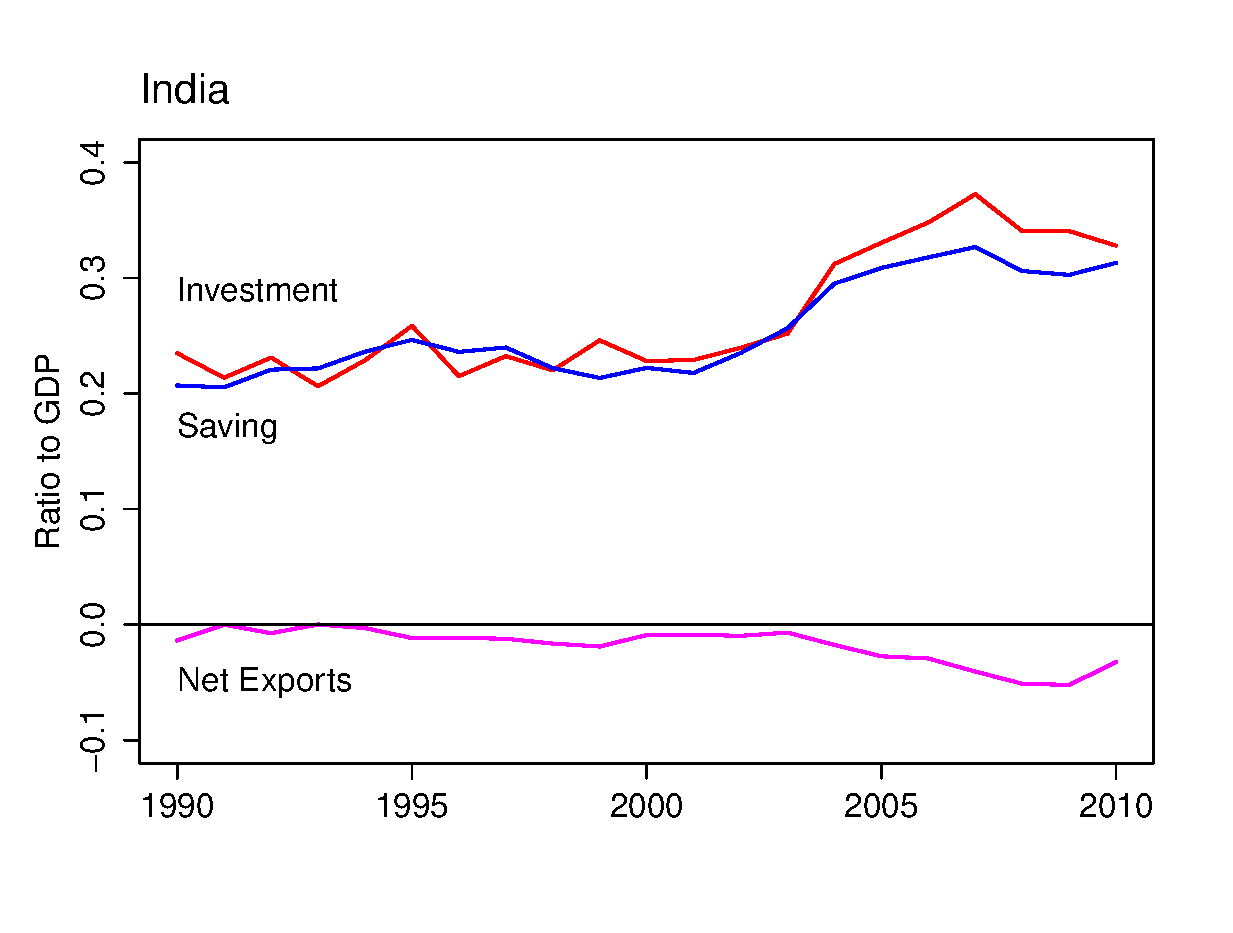
\includegraphics[scale=0.45]{India_shares.eps}
\end{center}

The figures tell us:
\begin{parts}
\part Saving and investment ``shares'' are significantly higher in China,
a difference of about 10\% of GDP.
\part Foreign sources of funds are reflected in net exports.
In China, capital is flowing out:  they're buying foreign assets.
In India, it capital is flowing in:  they're selling assets to the rest
of the world.
In both cases, the numbers are small relative to domestic saving.
\part Why?  Good question!
\end{parts}
\end{solution}

\end{questions}

\vfill \centerline{\it \copyright \ \number\year \
NYU Stern School of Business}

\end{document}

